\sect{5. How to play}

\begin{figure}[H]
\centering
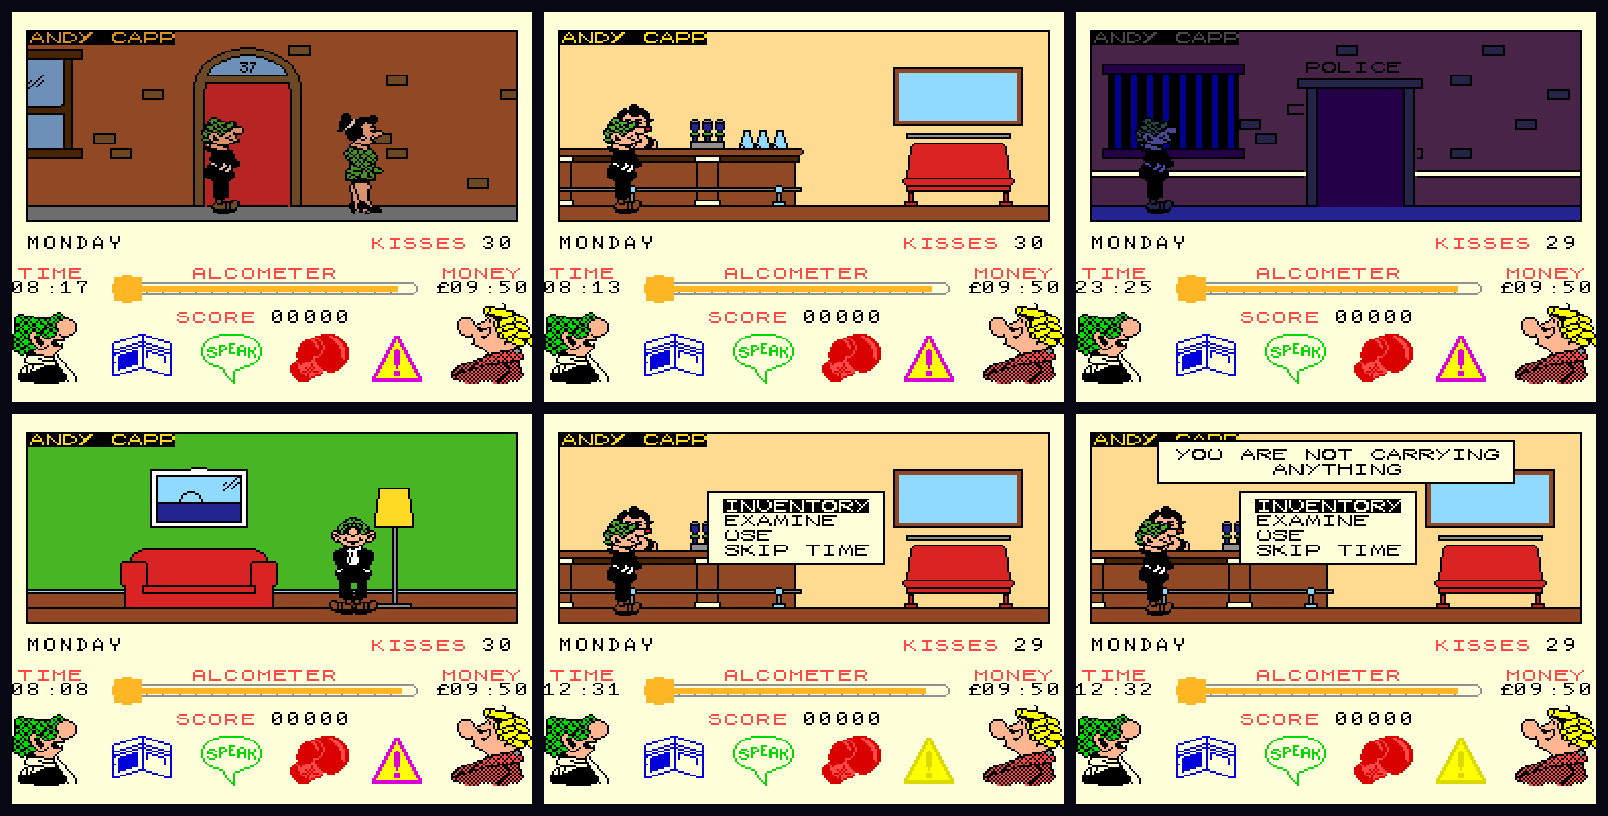
\includegraphics[width=\textwidth]{img/montage.png}
\caption{Andy's street, the pub, the police station at night, the front room, the ACTION menu and a message.}
\end{figure}

\textit{It's Monday morning and you're in a flat spin. Flo's demanding your dole cheque. She'll be off to her mother's if she doesn't get it soon. And who'll do the washing-up then? You'll need every ounce of your northern wile and charm to raise the cash to survive, one way or another. Maybe you can extract a quid or two from your friends? Or try your luck on the horses? But whatever you do, steer clear of the rent man and the local copper -- they're both after you with a vengeance!} (from the original instructions)

\textbf{The goal} is to get \textbf{the giro} (the dole cheque) and give it to Flo: with the giro in your pocket, stand next to her and use it (ACTION, USE). Getting there takes a chain of errands all over town.

\subsection*{The town}
Andy walks left and right along the streets; at the edge of the screen he goes on to the next one. At corners and at the doors of buildings, face them and press up. Two long streets are joined by side streets, with Andy's house (number 37), two \textit{Sparkling Ales} pubs, the police station, the court, the town hall, the employment exchange, the newsagent, the betting office and Fred's factory.

Buildings have \textbf{opening hours}: the pubs open from 11:00 to 15:00 and from 17:00 to 23:00; shops and offices from Monday to Saturday, 8:00 to 17:00, and close on Sunday. At night the streets get dark.

\subsection*{The people}
Walking around the streets are \textbf{Flo}, another \textbf{woman} with a ponytail, the \textbf{rent man} and several \textbf{policemen}. Inside the buildings there are people behind the counters: the barman, the newsagent, the clerk at the employment exchange, the police sergeant, the judge\ldots

\begin{itemize}
\item To speak to or fight someone you must \textbf{be touching them}, except for the people behind a counter.
\item People who are walking ignore you: first blow them a \textbf{kiss} (down). They stop for a while, stunned, and then you can talk to them. Kisses also stop a policeman so you can get away. They run out: watch the counter.
\end{itemize}

\subsection*{The icons}
Press \key{SPACE} and choose one of the four icons at the bottom:

\begin{description}
\item[WALLET (TRANSACT)] Buying and paying: a paper at the newsagent, a pint in the pub, the rent at the town hall, a bet at the betting office, an advance at the factory\ldots{} What is on offer depends on where you are. Andy starts with \pounds 9.50.
\item[SPEAK] Conversation and questions: \texttt{HAVE YOU SEEN MY RENT BOOK}, \texttt{HELLO}, \texttt{HAVE YOU SEEN MY GIRO}. Some places have questions of their own (the employment exchange, the factory\ldots).
\item[FIGHT] Sometimes getting into a scrap is the only way out. See section~7.
\item[ACTION] \texttt{INVENTORY} (what you carry), \texttt{EXAMINE} (look at an object), \texttt{USE} (use an object: drink the pint, give something to someone) and \texttt{SKIP TIME} (moves the clock on 4 hours, at the cost of a little alcohol).
\end{description}

Objects do not lie about on the floor: you buy them, you are given them, or you find them by doing the right thing in the right place.

\subsection*{The alcometer}
The alcometer bar goes down as time passes. \textbf{If it empties, the game is over.} It is topped up with a \textbf{pint}: buy it in the pub with the wallet and drink it \textbf{inside the pub} (ACTION, USE). Walk out into the street with the pint in your hand and the police are after you. When the bar is full, you have 30 kisses again.

\subsection*{Police, jail and the judge}
Andy is \textbf{wanted} if he fights or leaves the pub with the pint. While he is wanted, a policeman who touches him takes him on in a fight (unless you stopped him with a kiss). Lose a fight and you spend the night in the cells; the next morning the judge fines you \pounds 20: if you do not pay (or cannot), the game is over.

% ------------------------------------------------------------------
\sect{6. The status panel}

\begin{center}
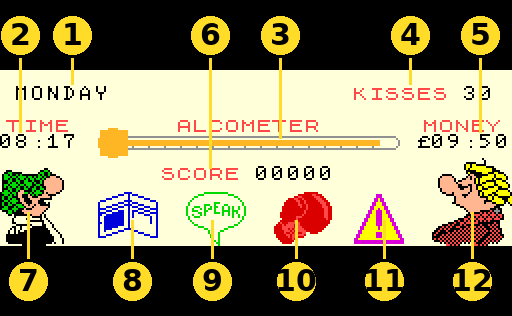
\includegraphics[width=0.9\textwidth]{img/hud.png}
\end{center}

\begin{tabularx}{\textwidth}{@{}clX@{}}
\toprule
\textbf{\tNo} & \textbf{\tElement} & \textbf{\tTellsYou}\\
\midrule
1 & Day & The day of the week. It changes at midnight.\\
2 & TIME & The time (00:00 to 23:59). A minute of game time lasts a second and a half.\\
3 & ALCOMETER & How much drink Andy has left. If it empties, the game is over.\\
4 & KISSES & The kisses you have left.\\
5 & MONEY & Your money, in pounds and pence.\\
6 & SCORE & The score: you earn it by fighting.\\
7 & Andy & Andy Capp.\\
8 & Wallet & TRANSACT icon: buying and paying.\\
9 & SPEAK & The speak icon.\\
10 & Glove & The fight icon.\\
11 & Sign & ACTION icon: objects and SKIP TIME. The chosen icon flashes.\\
12 & Flo & Flo, waiting for her money.\\
\bottomrule
\end{tabularx}

% ------------------------------------------------------------------
\sect{7. Scoring and the end}

\begin{itemize}
\item The \textbf{score} only goes up by fighting: every punch Andy lands scores points, and winning a fight gives a bonus. The fight is shown as a cloud of dust; luck decides it, punch by punch. Every punch you take lowers the alcometer, every one you land raises it a little.
\item \textbf{You win} when you give Flo the giro: \texttt{YOU HAVE WON} appears.
\item \textbf{You lose} if the alcometer empties, or if the judge fines you and you do not pay.
\item There is no day limit: the week goes on until you win or lose.
\end{itemize}

% ------------------------------------------------------------------
\sect{8. Tips}

\begin{itemize}
\item Keep your alcometer topped up -- the necessary is available from you-know-where, but only during opening hours.
\item Steer clear of the policeman -- you're on the wanted list.
\item If you fancy a flutter, remember you don't only get tips from the inlay card: read the racing paper.
\item After all, if things get desperate, you could always get a job.
\item Talk to everybody (blow a kiss first if they are walking) and ask about the giro and the rent book.
\item Some people are softened by a little present.
\item SKIP TIME helps you reach opening time, but it costs drink.
\end{itemize}

{\small The first four tips are the ones of the original instructions.}
